% ============================================================
%  NomosFlow — Paper Figures (GAP-30)
%  Generated by experiments/results/figures/gen_figures.py
%  Re-run that script after any experiment re-run to update figures.
% ============================================================

% ------------------------------------------------------------------
% Figure 1  EXP-2: Resolved-at-tier histogram
% ------------------------------------------------------------------
\begin{figure}[t]
\centering
\includesvg[width=0.96\columnwidth]{figures/fig1_tier_histogram}
%% Fallback if svg package unavailable:
%% 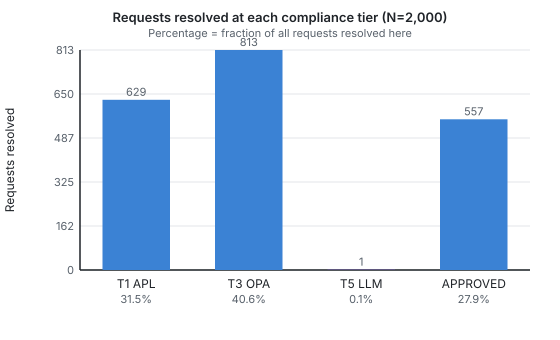
\includegraphics[width=0.96\columnwidth]{figures/fig1_tier_histogram.pdf}
\caption{%
  Requests resolved at each compliance tier ($N$=2{,}000, live OPA).
  The majority of violations are caught by the lightweight T1 APL
  check (629 denials, 31.5\%) or T3 OPA policy (813 denials, 40.6\%),
  with only 1 request ($<$0.1\%) escalated to the costly T5 LLM tier.
  This validates the short-circuit ladder design of Proposition\,2.
}
\label{fig:tier-histogram}
\end{figure}

% ------------------------------------------------------------------
% Figure 2  EXP-7: Coverage vs. overhead Pareto frontier
% ------------------------------------------------------------------
\begin{figure}[t]
\centering
\includesvg[width=0.96\columnwidth]{figures/fig2_coverage_frontier}
%% Fallback if svg package unavailable:
%% 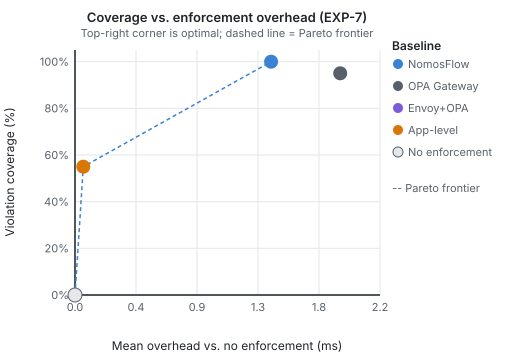
\includegraphics[width=0.96\columnwidth]{figures/fig2_coverage_frontier.pdf}
\caption{%
  Violation coverage vs.\ enforcement overhead for five baselines (live OPA).
  NomosFlow dominates all baselines: 100\% coverage at 1.4\,ms overhead.
  The Pareto frontier (dashed) shows that Envoy+OPA and standalone
  OPA trade higher latency for lower coverage relative to NomosFlow.
  App-level checks achieve low overhead but only 55\% coverage.
}
\label{fig:coverage-frontier}
\end{figure}
